\documentclass{standalone}
\usepackage{tikz}
\usetikzlibrary{patterns}
\usetikzlibrary{positioning}
\usetikzlibrary{patterns, positioning}
\usetikzlibrary{shapes.misc}
\usepackage[outline]{contour}
\contourlength{1.5pt} 


\begin{document}
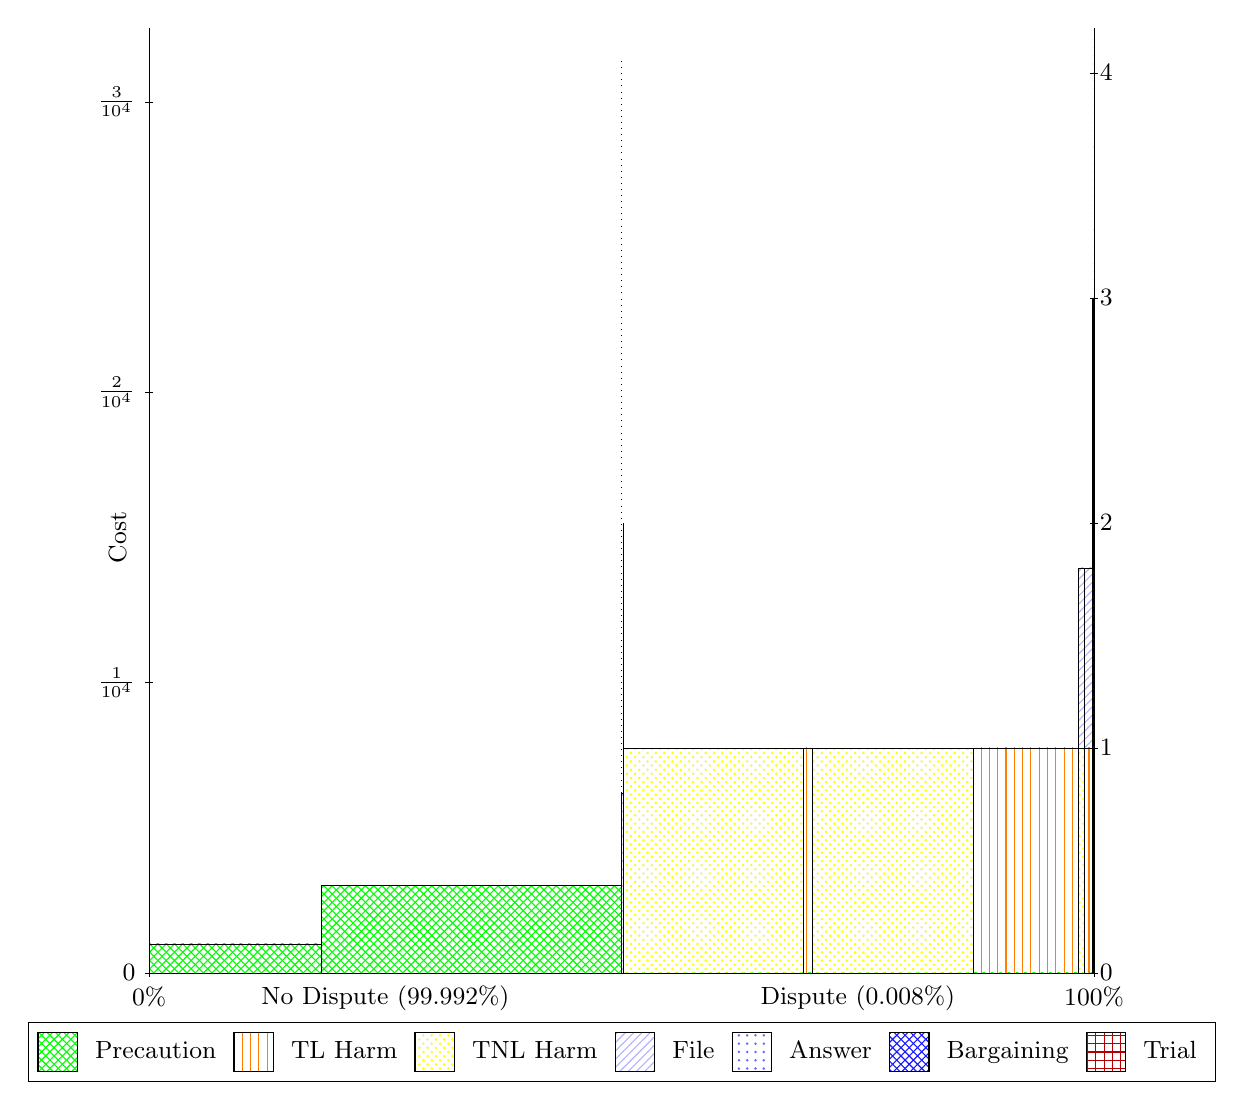
\begin{tikzpicture}
\draw[pattern=crosshatch, pattern color=green,draw=black,very thin] (1.5,2.5) rectangle (3.6907,2.8687);
\draw[pattern=crosshatch, pattern color=green,draw=black,very thin] (3.6907,2.5) rectangle (7.5,3.606);
\draw[pattern=crosshatch, pattern color=green,draw=black,very thin] (7.5,2.5) rectangle (7.5204,2.5);
\draw[pattern=north east lines, pattern color=blue!30,draw=black,very thin] (7.5,2.5) rectangle (7.5204,4.7857);
\draw[pattern=crosshatch, pattern color=green,draw=black,very thin] (7.5204,2.5) rectangle (7.5229,2.5);
\draw[pattern=north east lines, pattern color=blue!30,draw=black,very thin] (7.5204,2.5) rectangle (7.5229,4.7857);
\draw[pattern=dots,  pattern color=blue!60,draw=black,very thin] (7.5204,4.7857) rectangle (7.5229,5.9286);
\draw[pattern=crosshatch,      pattern color=blue!90,draw=black,very thin] (7.5204,5.9286) rectangle (7.5229,8.2143);
\draw[pattern=crosshatch, pattern color=green,draw=black,very thin] (7.5229,2.5) rectangle (9.8089,2.5);
\draw[pattern=crosshatch dots, pattern color=yellow,draw=black,very thin] (7.5229,2.5) rectangle (9.8089,5.3572);
\draw[pattern=crosshatch, pattern color=green,draw=black,very thin] (9.8089,2.5) rectangle (9.9187,2.5);
\draw[pattern=vertical lines, pattern color=orange,draw=black,very thin] (9.8089,2.5) rectangle (9.9187,5.3572);
\draw[pattern=crosshatch, pattern color=green,draw=black,very thin] (9.9187,2.5) rectangle (11.971,2.5001);
\draw[pattern=crosshatch dots, pattern color=yellow,draw=black,very thin] (9.9187,2.5001) rectangle (11.971,5.3572);
\draw[pattern=crosshatch, pattern color=green,draw=black,very thin] (11.971,2.5) rectangle (13.293,2.5001);
\draw[pattern=vertical lines, pattern color=orange,draw=black,very thin] (11.971,2.5001) rectangle (13.293,5.3572);
\draw[pattern=crosshatch, pattern color=green,draw=black,very thin] (13.293,2.5) rectangle (13.377,2.5);
\draw[pattern=crosshatch dots, pattern color=yellow,draw=black,very thin] (13.293,2.5) rectangle (13.377,5.3572);
\draw[pattern=north east lines, pattern color=blue!30,draw=black,very thin] (13.293,5.3572) rectangle (13.377,7.6429);
\draw[pattern=crosshatch, pattern color=green,draw=black,very thin] (13.377,2.5) rectangle (13.476,2.5);
\draw[pattern=vertical lines, pattern color=orange,draw=black,very thin] (13.377,2.5) rectangle (13.476,5.3572);
\draw[pattern=north east lines, pattern color=blue!30,draw=black,very thin] (13.377,5.3572) rectangle (13.476,7.6429);
\draw[pattern=crosshatch, pattern color=green,draw=black,very thin] (13.476,2.5) rectangle (13.494,2.5);
\draw[pattern=crosshatch dots, pattern color=yellow,draw=black,very thin] (13.476,2.5) rectangle (13.494,5.3572);
\draw[pattern=north east lines, pattern color=blue!30,draw=black,very thin] (13.476,5.3572) rectangle (13.494,7.6429);
\draw[pattern=dots,  pattern color=blue!60,draw=black,very thin] (13.476,7.6429) rectangle (13.494,8.7857);
\draw[pattern=crosshatch,      pattern color=blue!90,draw=black,very thin] (13.476,8.7857) rectangle (13.494,11.071);
\draw[pattern=crosshatch, pattern color=green,draw=black,very thin] (13.494,2.5) rectangle (13.498,2.5);
\draw[pattern=vertical lines, pattern color=orange,draw=black,very thin] (13.494,2.5) rectangle (13.498,5.3572);
\draw[pattern=north east lines, pattern color=blue!30,draw=black,very thin] (13.494,5.3572) rectangle (13.498,7.6429);
\draw[pattern=dots,  pattern color=blue!60,draw=black,very thin] (13.494,7.6429) rectangle (13.498,8.7857);
\draw[pattern=crosshatch,      pattern color=blue!90,draw=black,very thin] (13.494,8.7857) rectangle (13.498,11.071);
\draw[pattern=crosshatch, pattern color=green,draw=black,very thin] (13.498,2.5) rectangle (13.499,2.5);
\draw[pattern=crosshatch dots, pattern color=yellow,draw=black,very thin] (13.498,2.5) rectangle (13.499,5.3572);
\draw[pattern=north east lines, pattern color=blue!30,draw=black,very thin] (13.498,5.3572) rectangle (13.499,7.6429);
\draw[pattern=dots,  pattern color=blue!60,draw=black,very thin] (13.498,7.6429) rectangle (13.499,8.7857);
\draw[pattern=crosshatch,      pattern color=blue!90,draw=black,very thin] (13.498,8.7857) rectangle (13.499,11.071);
\draw[pattern=grid,            pattern color=red!70!black,draw=black,very thin] (13.498,11.071) rectangle (13.499,14.5);
\draw[pattern=crosshatch, pattern color=green,draw=black,very thin] (13.499,2.5) rectangle (13.5,2.5);
\draw[pattern=vertical lines, pattern color=orange,draw=black,very thin] (13.499,2.5) rectangle (13.5,5.3572);
\draw[pattern=north east lines, pattern color=blue!30,draw=black,very thin] (13.499,5.3572) rectangle (13.5,7.6429);
\draw[pattern=dots,  pattern color=blue!60,draw=black,very thin] (13.499,7.6429) rectangle (13.5,8.7857);
\draw[pattern=crosshatch,      pattern color=blue!90,draw=black,very thin] (13.499,8.7857) rectangle (13.5,11.071);
\draw[pattern=grid,            pattern color=red!70!black,draw=black,very thin] (13.499,11.071) rectangle (13.5,14.5);
\draw[black,very thin] (1.5,2.5) -- (1.5,14.5);
\node[font=\small,rotate=90,text=black, anchor=center] at (1.1, 8.0298) {Cost};
\draw[black,very thin] (1.45,2.5) -- (1.55,2.5);
\node[font=\small,text=black, anchor=east] at (1.45, 2.5) {0};
\draw[black,very thin] (1.45,6.1865) -- (1.55,6.1865);
\node[font=\small,text=black, anchor=east] at (1.45, 6.1865) {$\frac{1}{10^{4}}$};
\draw[black,very thin] (1.45,9.8731) -- (1.55,9.8731);
\node[font=\small,text=black, anchor=east] at (1.45, 9.8731) {$\frac{2}{10^{4}}$};
\draw[black,very thin] (1.45,13.56) -- (1.55,13.56);
\node[font=\small,text=black, anchor=east] at (1.45, 13.56) {$\frac{3}{10^{4}}$};

\draw[black,dotted,very thin] (7.5,2.86) -- (7.5,14.14);
\draw[black,very thin] (13.5,2.5) -- (13.5,14.5);
\draw[black,very thin] (13.45,2.5) -- (13.55,2.5);
\node[font=\small,text=black, anchor=west] at (13.45, 2.5) {0};
\draw[black,very thin] (13.45,5.3571) -- (13.55,5.3571);
\node[font=\small,text=black, anchor=west] at (13.45, 5.3571) {1};
\draw[black,very thin] (13.45,8.2143) -- (13.55,8.2143);
\node[font=\small,text=black, anchor=west] at (13.45, 8.2143) {2};
\draw[black,very thin] (13.45,11.071) -- (13.55,11.071);
\node[font=\small,text=black, anchor=west] at (13.45, 11.071) {3};
\draw[black,very thin] (13.45,13.929) -- (13.55,13.929);
\node[font=\small,text=black, anchor=west] at (13.45, 13.929) {4};

\draw[black,very thin] (1.5,2.5) -- (13.5,2.5);
\draw[black,very thin] (1.5,2.45) -- (1.5,2.55);
\node[font=\small,text=black, anchor=north] at (1.5, 2.45) {0\%};
\draw[black,very thin] (13.5,2.45) -- (13.5,2.55);
\node[font=\small,text=black, anchor=north] at (13.5, 2.45) {100\%};

\node[font=\small,text=black,anchor=south] at (4.5, 1.9) {No\ Dispute\ (99.992\%)};
\node[font=\small,text=black,anchor=south] at (10.5, 1.9) {Dispute\ (0.008\%)};
\draw (7.5,2.5) node (B) {};
\begin{scope}[align=center]
\matrix[scale=0.5,draw=black,below=0.5cm of B,nodes={draw},column sep=0.1cm]{
\node[rectangle,draw,minimum width=0.5cm,minimum height=0.5cm,pattern=crosshatch, pattern color=green]{}; & \node[draw=none,font=\small,text=black]{Precaution}; &
\node[rectangle,draw,minimum width=0.5cm,minimum height=0.5cm,pattern=vertical lines, pattern color=orange]{}; & \node[draw=none,font=\small,text=black]{TL Harm}; &
\node[rectangle,draw,minimum width=0.5cm,minimum height=0.5cm,pattern=crosshatch dots, pattern color=yellow]{}; & \node[draw=none,font=\small,text=black]{TNL Harm}; &
\node[rectangle,draw,minimum width=0.5cm,minimum height=0.5cm,pattern=north east lines, pattern color=blue!30]{}; & \node[draw=none,font=\small,text=black]{File}; &
\node[rectangle,draw,minimum width=0.5cm,minimum height=0.5cm,pattern=dots,  pattern color=blue!60]{}; & \node[draw=none,font=\small,text=black]{Answer}; &
\node[rectangle,draw,minimum width=0.5cm,minimum height=0.5cm,pattern=crosshatch,      pattern color=blue!90]{}; & \node[draw=none,font=\small,text=black]{Bargaining}; &
\node[rectangle,draw,minimum width=0.5cm,minimum height=0.5cm,pattern=grid,            pattern color=red!70!black]{}; & \node[draw=none,font=\small,text=black]{Trial}; \\\\
};\end{scope}

\end{tikzpicture}
\end{document}